\begin{figure*}[hbtp]
  \centering
  \subfigure[Results of each graph]{
    \label{fig:louvain--all}
    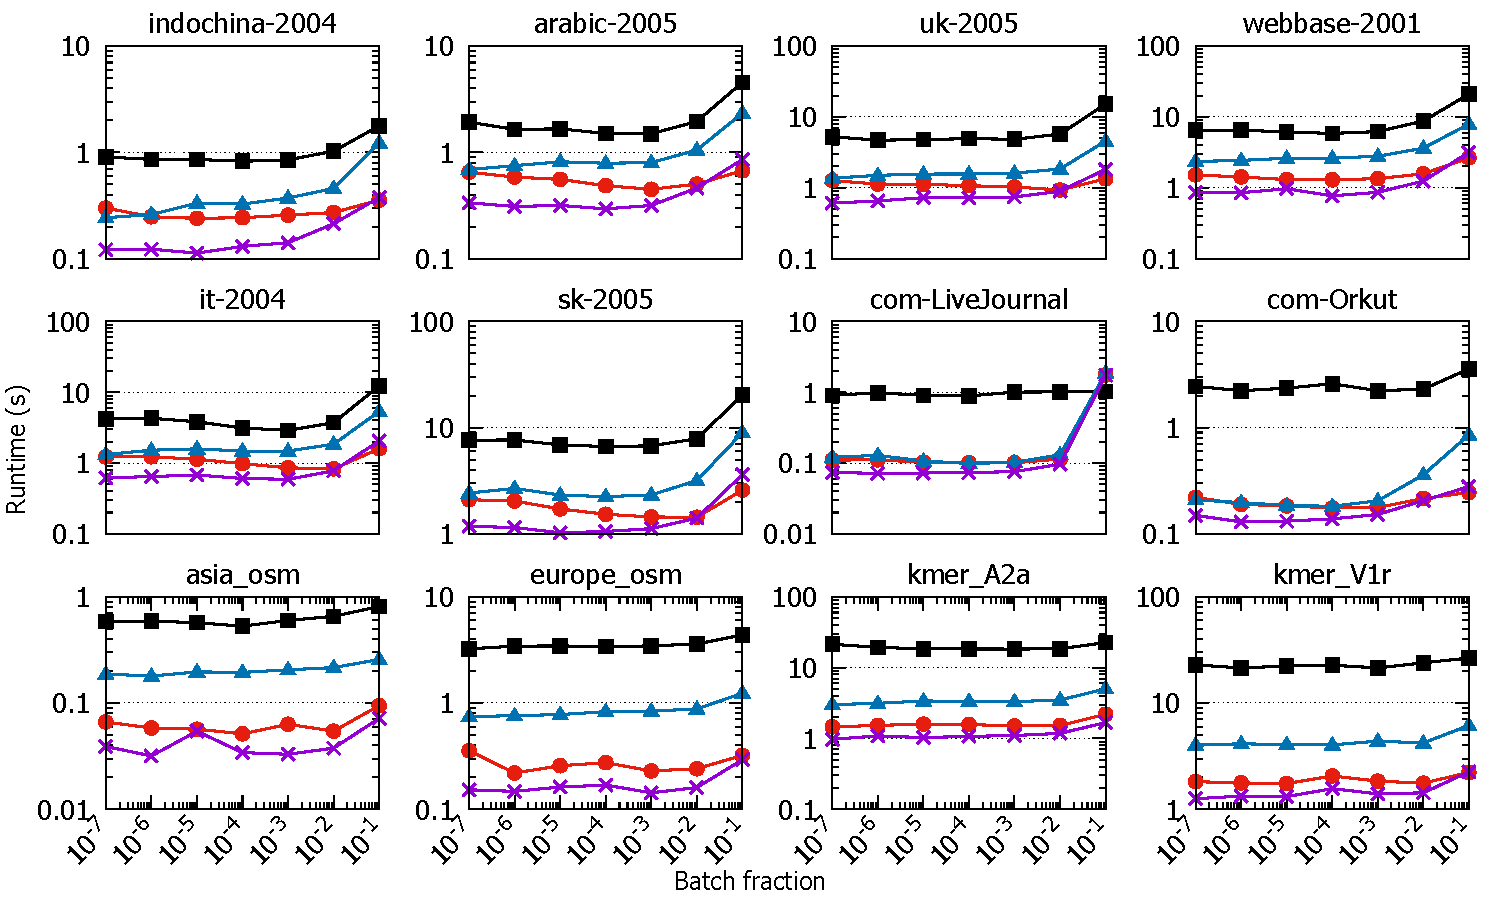
\includegraphics[width=0.58\linewidth]{out/louvain-all.pdf}
  }
  \subfigure[Overall result]{
    \label{fig:louvain--am}
    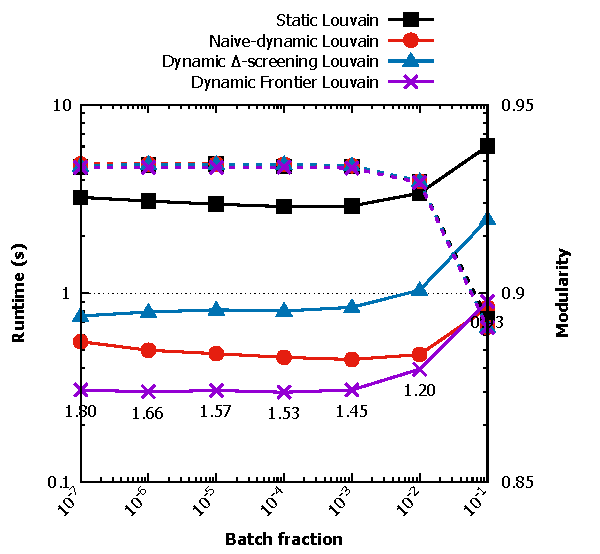
\includegraphics[width=0.38\linewidth]{out/louvain-am.pdf}
  } \\[-2ex]
  \caption{Time taken (solid lines), and modularity of communities obtained (dashed lines) along the right Y-axis, with \StaLou{}, \NaiLou{}, \DelLou{}, and \FroLou (Algorithm \ref{alg:louvain}) on batch updates of increasing size from $10^{-7} |E|$ to $0.1 |E|$. Note that both axes are logarithmic. Speedup of \FroLou{} with respect to \NaiLou{} is labeled.}
  \label{fig:louvain}
\end{figure*}
